\chapter{Software}

To implement the HLI functionality Python was chosen for its ease of writing as well as its extensive library of predefined functions. This enables the programmer to utilize highly complex functions through simple and  On of these libraries is NumPy, which enables the user to define vectors and matrices and do calculations with these, in the same way Matlab does. This made it easy to port Matlab code from simulation to actual implementation. Another library is the MatPlotLib library. This eased the path planning implementation, as it was possible to plot the result of the proposed algorithms during testing. Further, another Python library allowed the script to easily access the OpenStreetMap API and retrieve the relevant data.

The LLI functionality was implemented in C as this is the primary embedded programming language with which the project group has experience.

\section{System Description}

The HLI consists of 3 main modules and an additional simulator module, which is not rqeuired for the embedded application.

The main module of the software is the Ship Class and its function definitions.
The Ship Class itself represents an emph{actor} in the system. A Ship Object has individual dynamic model, controller and objective. Each Ship Object can plan its own waypoints, navigate trough them using their own sensor data and log informations.

\begin{center}
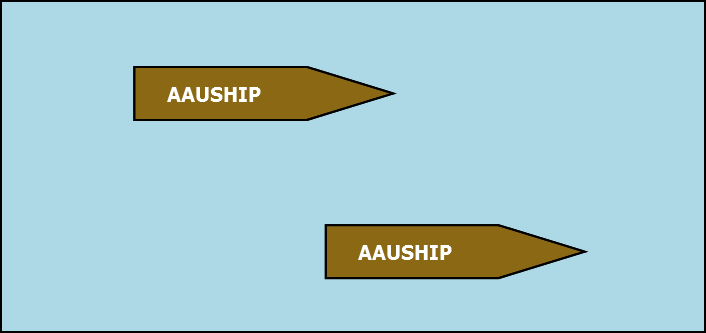
\includegraphics[width = 0.5\textwidth]{img/HLIFigures/ActorModel/Actor-model0.png}
\end{center}

A Ship Object requires auxillary Classes and Functions. The two side-modules of the system are the ObjectLibrary and FunctionLibrary. These Libraries store Classes and Functions, which are not directly connected to the physical behaviour of the ship, but provide an essential support for the Path Planning and Navigation control.

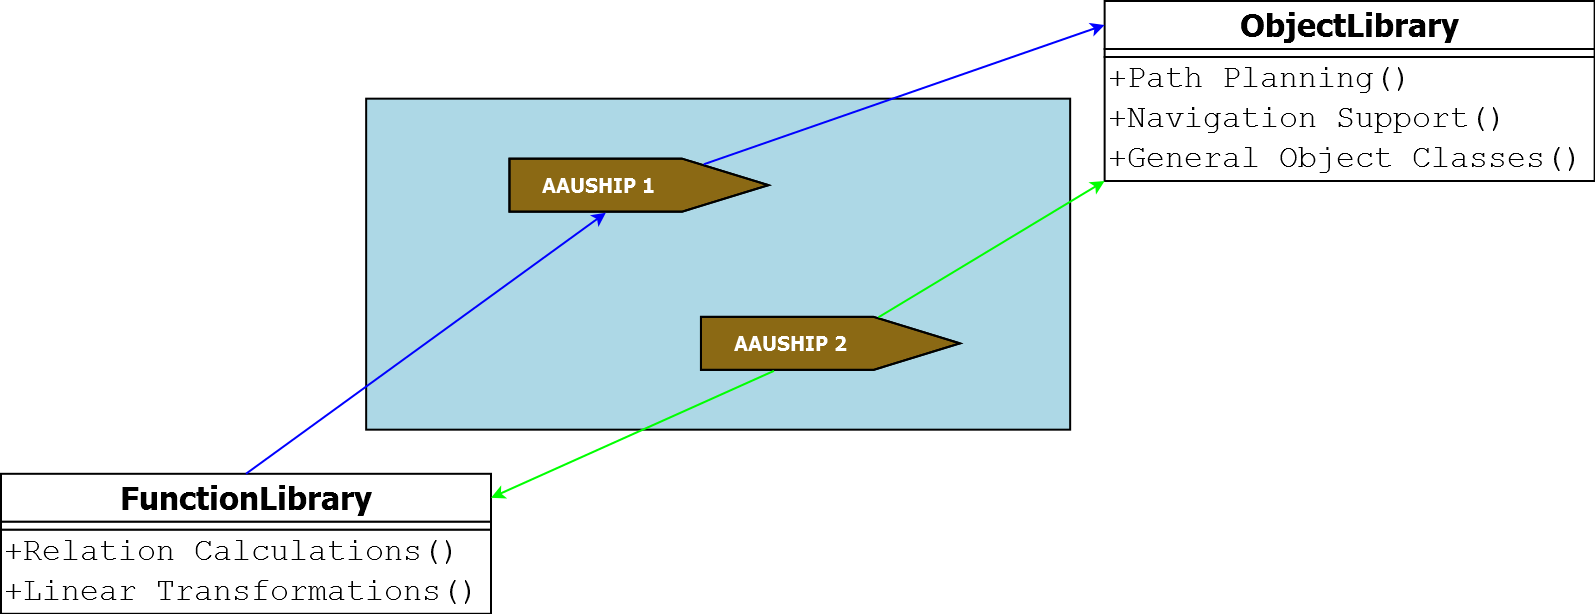
\includegraphics[width = \textwidth]{img/HLIFigures/ActorModel/Actor-model1.png}


Each ship calculates its own \emph{Waypoints}, depending on their individual capabilities and inputs.
There is a possibility for the ships to communicate trough a wireless channel with each other directly or trough a nearby mothership/computer, in order to share position data (to avoid collisions), or distribute the Path Planning tasks for enhanced computation power.

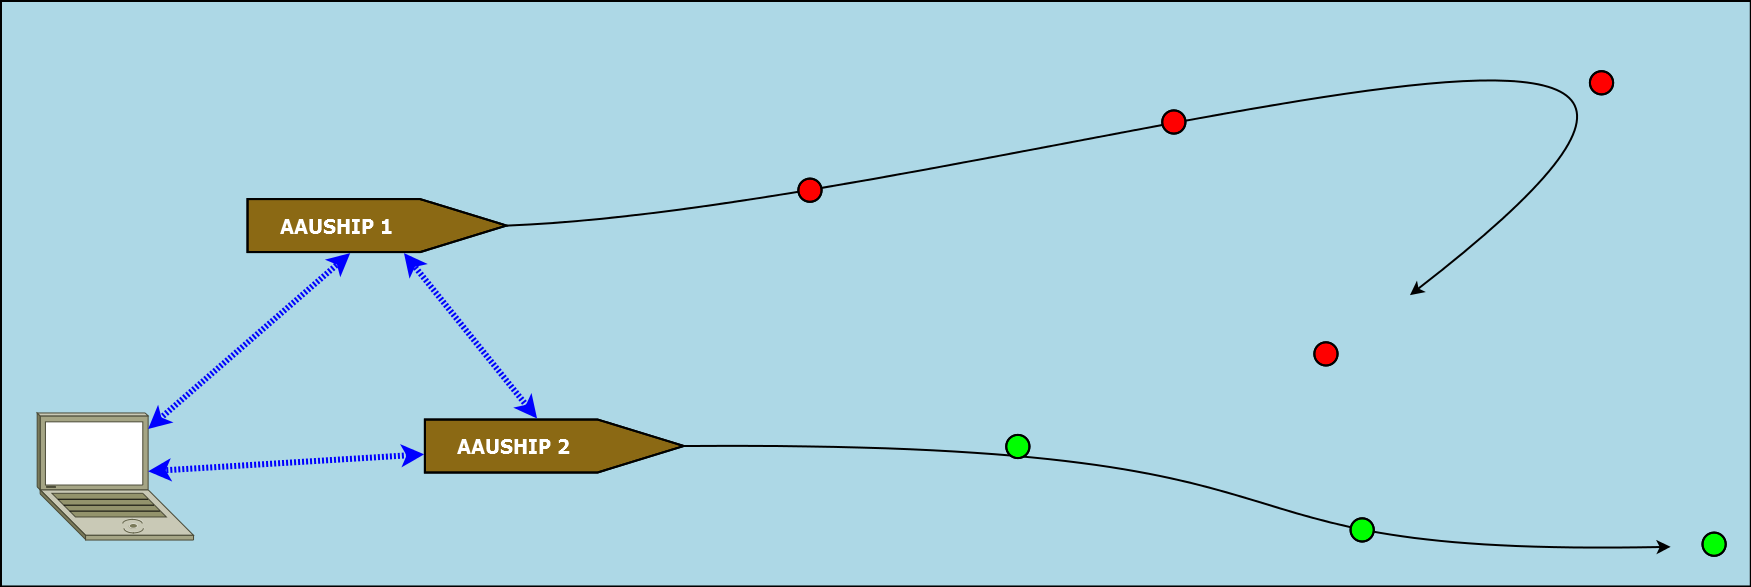
\includegraphics[width = \textwidth]{img/HLIFigures/ActorModel/Actor-model2.png}


The additional simulator module is an extension of the \emph{Ship Object}. In Simulation mode, to each \emph{Ship} belongs a \emph{Simulator}, simulating its interface communication and dynamic behaviour. The design of the simulator was led by two objectives:
\begin{itemize}
\item The \emph{Simulation} and the \emph{Embedded} application must run with the absolutely same \emph{Ship Class Module}
\item The simulator must predict the behaviour of the system well, but must be using a different model than the inner \emph{State Estimator Kalman Filter} of the ship
\item The simulator must be completely independent from the simulated system, except for the actuator values of the Ship.
\end{itemize}

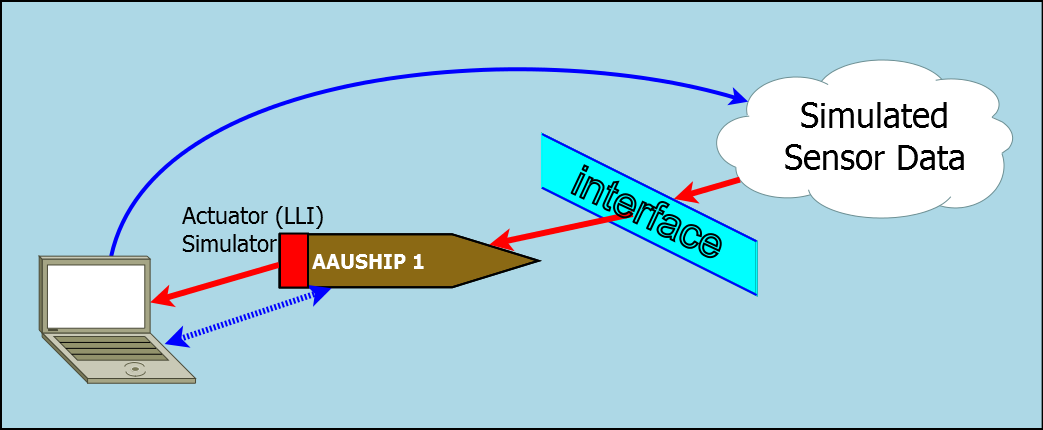
\includegraphics[width = \textwidth]{img/HLIFigures/ActorModel/SimModel.png}

Because of the predefined objectives above, the flowchart of the simulated and the actual task only slightly differs (Appendix)

%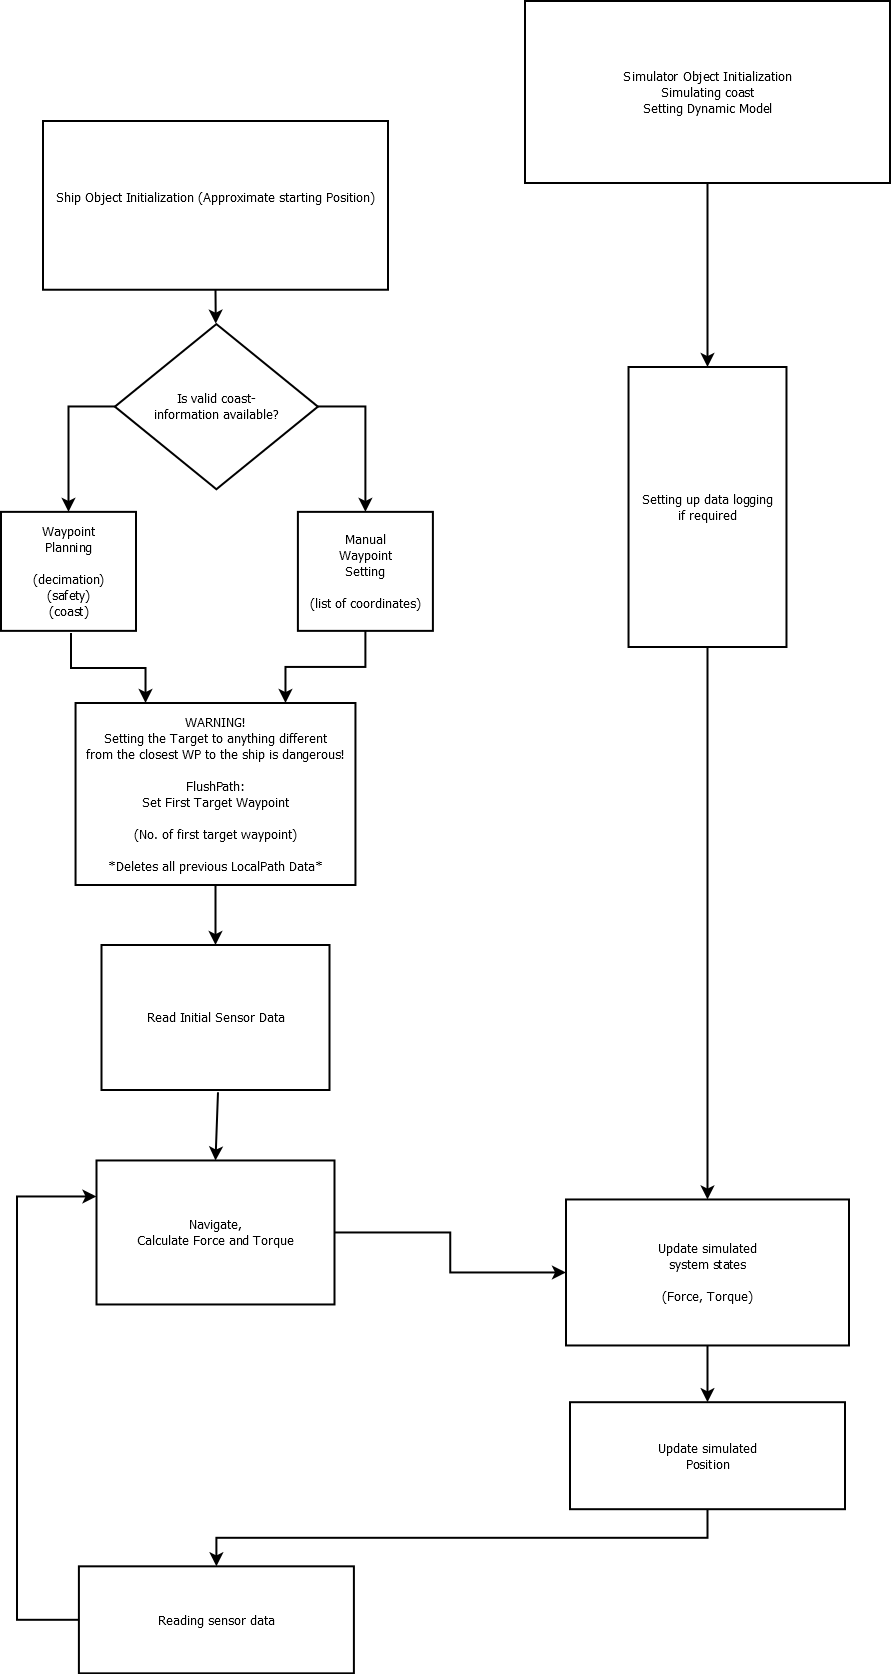
\includegraphics[width = \textwidth]{img/HLIFigures/System-Simulation_Interactions.png}

%The differences are kept on the right side of the Flowchart:

%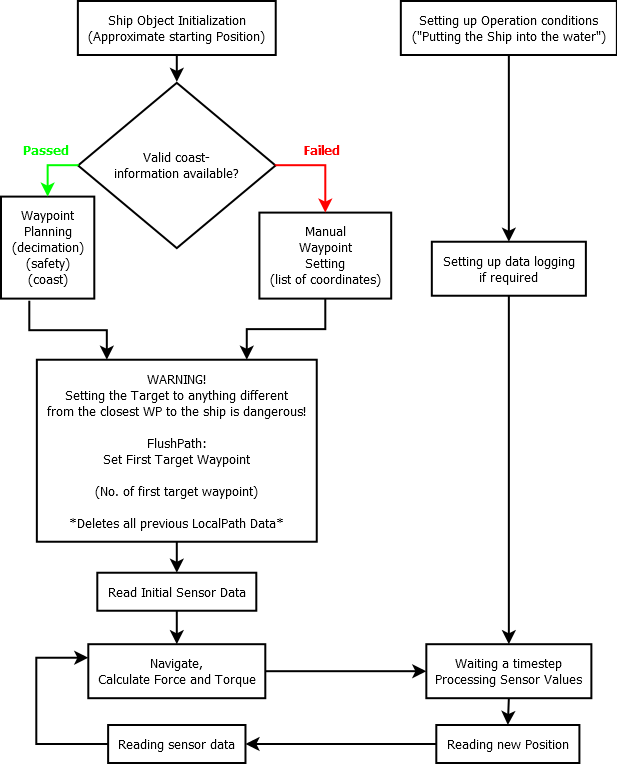
\includegraphics[width = \textwidth]{img/HLIFigures/System-World_Interactions.png}

\section{Course keeping control}

The Course-keeping control is responsible for keeping the ship on-course during Autonomous navigation.

The general idea is to have a state-space control algorithm in infinite loop as the main task. The control parameterization is based on the ship model, measurements and identification.
The program controls the ship along the specified path. If there is no next sub-\emph{Waypoint} or local path specified, the HLI calls the path planning methods for the next \emph{Waypoint}, then the procedure starts again from the beginning. If there are no more \emph{Waypoints}, the ship returns to the first \emph{Waypoint}, or to the starting coordinates specified in a subfunction of the Ship class.

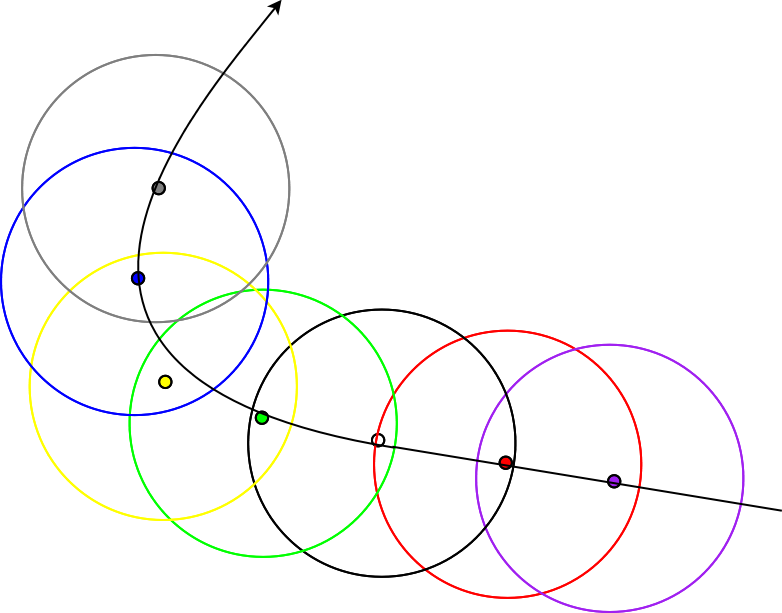
\includegraphics[width = \textwidth]{img/HLIFigures/SWPNavigationConcept.png}

Using Sub-\emph{Waypoints} instead of a full path line makes the navigation much easier. In open water there is significant sideways-motion caused by wind, ocean currents and waves, so staying perfectly true to a predefined path line is extremely difficult.
Instead, by using a series of Sub-\emph{Waypoints}, the navigation of the ship resembles to a series of Buoys guiding trough hazardous waters. The Ship approaches each Sub-\emph{Waypoint} in a predefined order and turns to the next, when the ''buoy´´ is close enough.
The characteristics of the navigation and course can be varied only by changing the definition of the Sub-\emph{Waypoints}, setting optimal parameters for different locations and settings.

\section{\emph{Waypoint} Planning}

The \emph{Waypoint}-planning system provides the basic routing for the autonomous navigation system.
The purpose of the \emph{Waypoint}-planning is to set key coordinates that the ship must approach, either for strictly defined reasons or to keep the ship away from forbidden or dangerous areas (like the coast or an island)

There are two possibilities to set a collection of \emph{Waypoints}: The operator can either manually set them, based on the GPS coordinates of the \emph{Waypoints}, or by inputting a coastline data series is a specified data type. The coast input format is a series of perpendicular distances measured from a line parallel to the coast. The coast input can be generated based on freely available map data (Openstreetmap).
The automatic \emph{Waypoint} planner divides the coast to smaller parts, based on the required oceanography definition. For each segment a minimum approach distance is calculated, and the \emph{Waypoint} planner defines a set of \emph{Waypoints} along the path in a snake way, or in any other predefined setting. The figure below shows a simulation of an oceanography task using automatic \emph{Waypoint} planning. All values in meters.
After the ship visited all of the \emph{Waypoints}, it returns to the first \emph{Waypoint}, or to a specified return position.

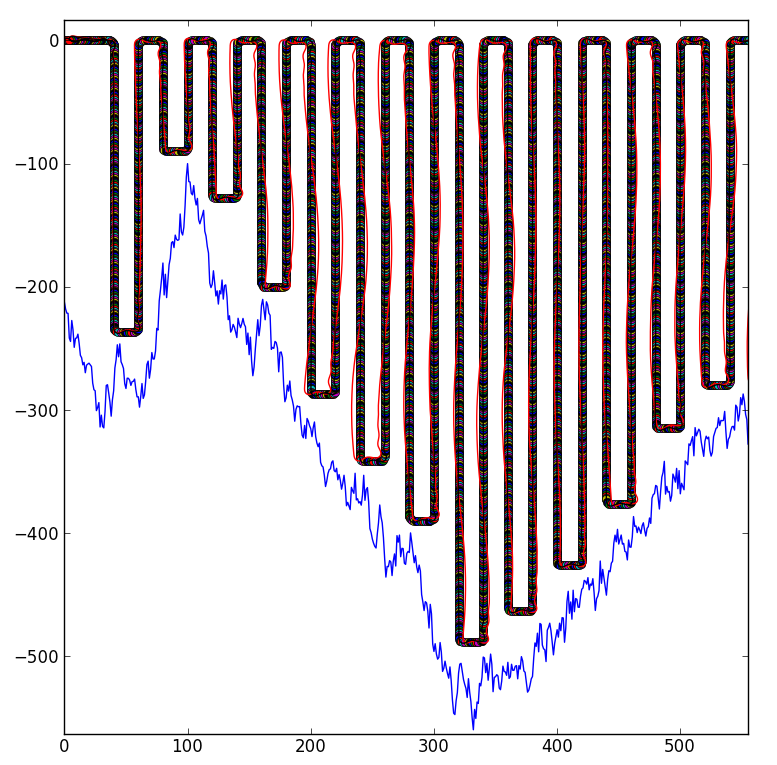
\includegraphics[width = \textwidth]{img/LocalPlannerFigures/Auto_WP_Planning.png}

Why are we using it?
The need for a basic \emph{Waypoint}-planner is essential, but optimizing it was not a high priority task. To test the prototype, a series of manually set \emph{Waypoints} are adequate.

\section{Local Planner}

The Local planner is responsible for planning a segment of the path, in order to supply the controller with a series of Sub-\emph{Waypoints}. The Local path should result in a set of points, which are lined up smoothly enough for the ship to sail through them with the reference speed.

The path can be divided to a straight line and a turning sub-path. The combination of a straight path and a turn is a Path Segment. The local planner calculates a Path Segment from the current position to the end of the turn at the next Turning \emph{Waypoint} (Footnote: If three \emph{Waypoints} are in a line, the angle at the second is $\pi$, therefore it is not a turning \emph{Waypoint}), based on the \emph{Waypoint} after the Turning \emph{Waypoint} as well.

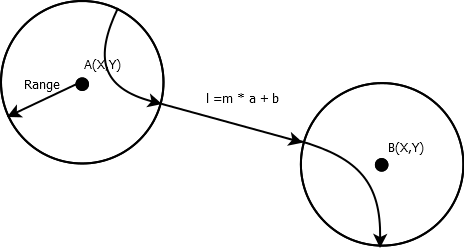
\includegraphics[width = \textwidth]{img/LocalPlannerFigures/StraightRoute.png}

Calculating the smooth set of points for the turn:
The initial idea was to use a pre-generated Euler-spiral or simple arc line, the program determines the required arc length and applies linear transformations to resize and rotate the path coordinates, thus creating a smooth path.
The initial idea was dropped after the following considerations:
\begin{itemize}
\item Storing the full path coordinates is memory-consuming. Also, the path has either low resolution or the linear transformation would be CPU-heavy
\item The path would be smooth but would not have optimal parameters \ldots
\end{itemize}

The new idea is originated from: Koml\'osi Istv\'an: Mobilis robotok auton\'om navig\'aci\'oja mozg\'o akad\'alyok elker\"ul\'es\'evel (English version: Istv\'an Koml\'osi and B\'alint Kiss: Motion planning for multiple mobile robots using time-scaling).
The concept is to determine the maximum possible path curvature that the robot can handle. This is based on the Sigma and Kappa values of the Ship, where sigma is a function of the maximum speed of Torque change, and kappa is the maximum curvature of the path at a given speed. The local path is generated in a specific way that the robot will always turn with the maximum possible curvature at the current speed, thus staying the closest to the \emph{Waypoint} without losing speed. There is a threshold turn-angle, which determines if the robot requires only two identical Euler-spiral paths to turn or an arc path that has the maximum curvature, with two Euler spiral paths leading in or out.
In order to create the path the algorithm calculates 5 or 3 (depending on the threshold) key points and fits a Hermite-poly onto them. From this point on the local path in the given range is determined by these points only, thus saving memory and CPU time, while calculating a better path.
\begin{center}
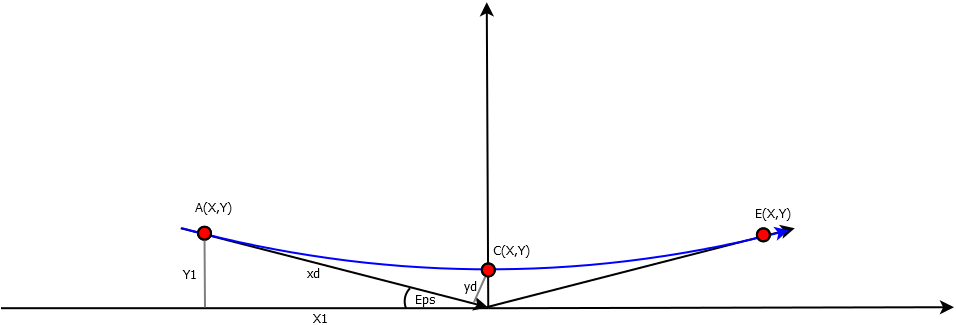
\includegraphics[width = \textwidth]{img/LocalPlannerFigures/3Points.png}
The calculation of the 3 key-points if $\epsilon < \epsilon_{max}$ (no circular path component is needed)

$$ \sigma = \frac{\beta_max}{v^2} $$
$$x_d = \frac{\pi}{\sigma} * C_F(\epsilon)$$
$$y_d = \frac{\pi}{\sigma} * S_F(\epsilon)$$

Where $C_F$ and $S_F$ are the normalized Fresnel-integral functions.

$$X_1 = x_d * cos(\epsilon) + y_d * sin(\epsilon)$$
$$Y_1 = X_1 * tan(\epsilon)$$

$$A = (-X_1, Y_1)$$
$$C = (0, \frac{y_d}{cos(\epsilon)})$$
$$E = (X_1, Y_1)$$

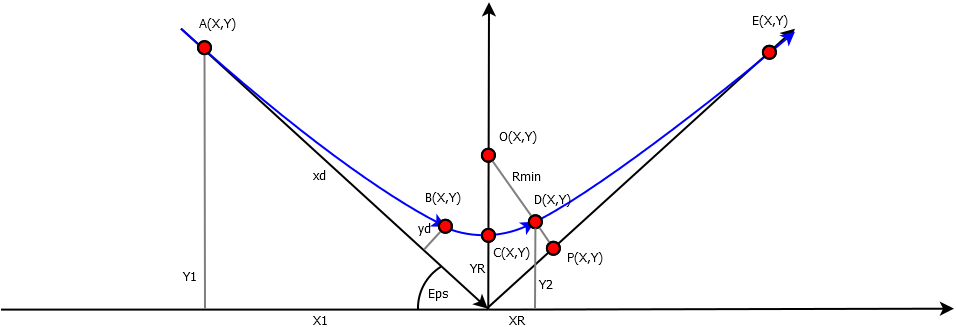
\includegraphics[width = \textwidth]{img/LocalPlannerFigures/5Points.png}
The calculation of the 5 key-points if $\epsilon > \epsilon_{max}$ (a circular path component is needed)

$$ \sigma = \frac{\beta_max}{v^2} $$
$$x_d = \frac{\pi}{\sigma} * C_F(\epsilon)$$
$$y_d = \frac{\pi}{\sigma} * S_F(\epsilon)$$

Where $C_F$ and $S_F$ are the normalized Fresnel-integral functions.

$$X_R = R_{min} * sin(\epsilon - \epsilon_{max})$$
$$P_X = X_R + y_d * sin(\epsilon)$$
$$X_1 = P_X + x_d * cos(\epsilon)$$
$$Y_1 = X_1 * tan(\epsilon)$$
$$P_y = Y_1 - x_d * sin(\epsilon)$$
$$Y_2 = P_y + y_d * cos(\epsilon)$$
$$O_Y = R_{min} * cos(\epsilon-\epsilon_{max) + Y_2}$$
$$R_Y = O_Y - R_{min}$$
$$X_2 = X_R$$

$$A = (-X_1, Y_1)$$
$$B = (-X_2, Y_2)$$
$$C = (0, Y_R)$$
$$D = (X_2, Y_2)$$
$$E = (X_1, Y_1)$$

\end{center}
The Hermite-polinom is used to populate the path with a number of points, depending on the predefined conditions. The resulting set of points is transformed to its correct place by a transformation matrix in the Local Frame, around the Turning \emph{Waypoint}.

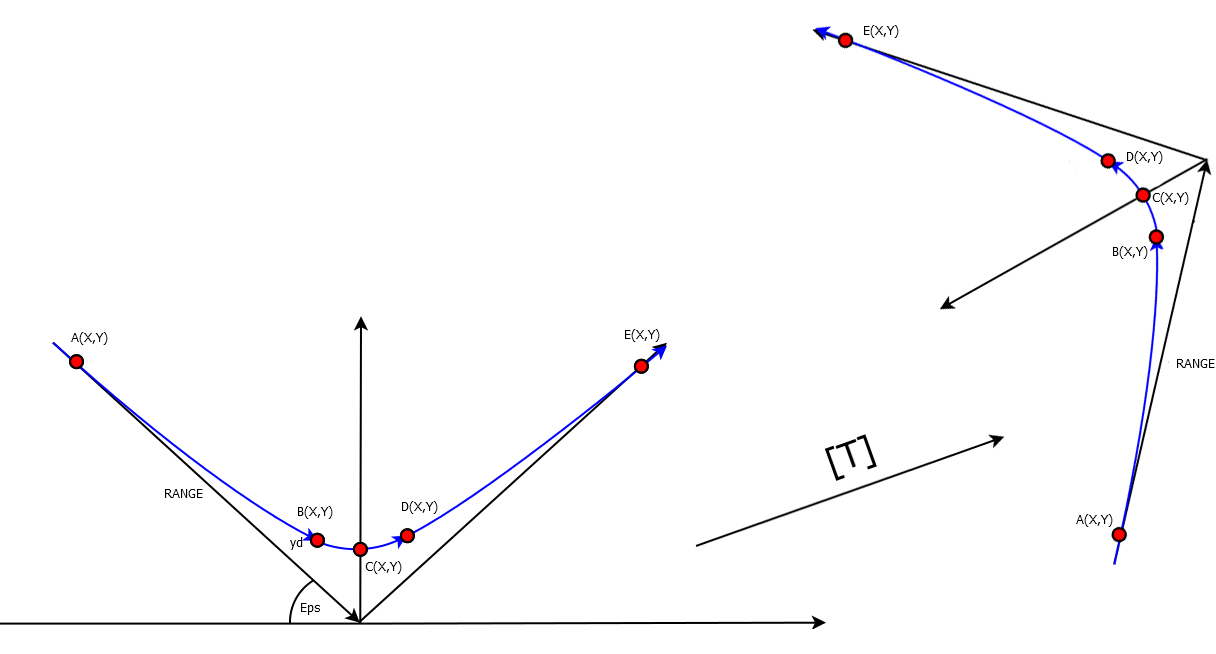
\includegraphics[width = \textwidth]{img/LocalPlannerFigures/PositioningTurn.png}

The considerations behind this path planning method were based on the following conditions:
\begin{itemize}
\item The ship must be able to output the next \emph{Waypoint} quickly, therefore calculating the whole path line in a single batch was to be avoided
\item The \emph{Waypoints} of the ship are subject to possible changes. Re-calculating the whole path every time a \emph{Waypoint} is changed is very consuming
\item The Ship is subject to unpredictable outside forces. Every path-segment is to be computed to be optimal, based on the actual, not the ideal prepared position
\item The local planning should be as efficient as possible. Planning every Sub-\emph{Waypoint} individually is a lot less effective than planning them in a batch \ldots
\end{itemize}

The Aurea mediocritas\footnote[1]{Golden mean} lies in dividing the path to segments, and planning the Sub-\emph{Waypoints} of each segment in a batch.
